\documentclass[14pt,a4paper]{book}

\usepackage[utf8]{inputenc}
\usepackage[german,english,russian]{babel}
\usepackage[unicode]{hyperref}
% \hypersetup{unicode=true}

\usepackage{graphicx}
\usepackage{xcolor}

\newcommand{\DE}[1]{\textcolor{green}{#1}}
\newcommand{\RU}[1]{\textcolor{red}{#1}}
\newcommand{\TRpart}[2]{\chapter{#2 /#1/}}
\newcommand{\TRchapter}[2]{\chapter{#2 /#1/}}
\newcommand{\TRsection}[2]{\chapter{#2 /#1/}}
\newcommand{\TRsubsection}[2]{\chapter{#2 /#1/}}

\newcommand{\file}[1]{\textbf{#1}}

\title{Стойка ЧПУ KOSY и NCCAD7}
\author{перевод Dmitry Ponyatov <dponyatov@gmail.com>}

\begin{document}

\maketitle

\RU{Кривой перевод оригинальной документации из поставки учебного комплекта станков
WABECO~--- файлы \file{nccad7.chm} и \file{ZSE3Help.chm} с немецкого.
Комплектность поставки документации от ecoinvent хромает, могли бы хотя бы
английский вариант положить как опцию.}

\tableofcontents

\TRpart{NCCAD7}{NCCAD7}

\DE{Hilfethemen für nccad7 - 18. 02. 2005}
\RU{Справка для nccad7 - 18 02, 2005}
\DE{Überarbeitet: August 2002}
\RU{Редакция: Август 2002}

\TRchapter{Suchen von Worten}{Поиск по словам}

\bigskip 

\DE{Angenommen Sie möchten eine nähere Erklärung zum Begriff "Nullpunkt".}
\RU{Вероятно Вы хотели бы более точное определение термина
"нулевая точка".}
\DE{Innerhalb aller Hilfethemen kommt dieser Begriff auf mehreren Seiten vor.}
\RU{Кажется что этот термин используется на каждой странице этого
документа.}
\DE{Um diese Seiten - und die zugehörigen Textstellen zu finden gibt es die
Funktion "Suchen".}
\RU{Чтобы найти такие страницы и соответствующие места в тексте,
существует функция ``Поиск''}
\DE{Sie gehen folgendermaßen vor:}
\RU{Он используется следующим образом:}
\begin{enumerate}
  \item Öffnen Sie die Karteikarte \textbf{Suchen} durch Klick auf den Reiter
  "Suchen".
  \item Geben Sie im \textbf{Feld Suchbegriff} das Suchwort komplett ein. 
\begin{enumerate}
  \item Achten Sie auf Rechtschreibung. 
  \item Die Klein/Großschreibung wird in der Suchfunktion nicht beachtet, z.B.
  \item kann eingegeben werden "nullpunkt" oder "Nullpunkt".
  \item Schon einmal eingegebene Suchworte sind über das PullDown-Menü wieder
  aufrufbar (Pfeil nach unten).
  \item In den Suchbegriff können logische Verknüpfungen eingebaut werden, die
Sie über den Button "Pfeil nach rechts" neben dem Eingabefeld erreichen.
\end{enumerate}
  \item Klicken Sie auf "Themen auflisten". Eine Liste mit den Seiten, in denen
das Suchwort mindestens einmal vorkommt, erscheint.
  \item Wählen Sie durch Doppelklick eine dieser Seiten aus. In der
dargestellten Seite werden die gefundenen Textstellen markiert. Durch Scrollen können
 Sie die Textstellen auffinden. (Siehe Bild, unterer Teil).
\end{enumerate}

\bigskip

Das folgende Bild gibt einen Überblick über die verschiedenen Phasen des Suchens:

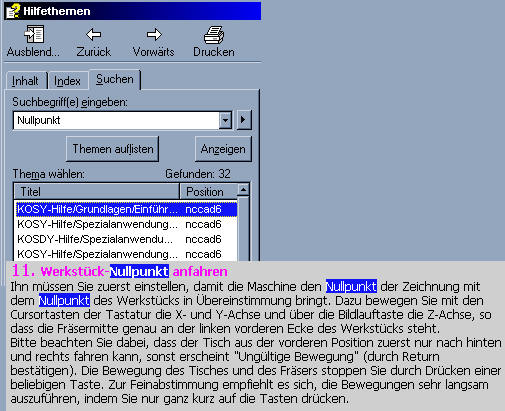
\includegraphics{pic/Suche1.png}

\TRchapter{Das Indexregister}{Индексный регистр}

\DE{Falls Sie mehr Informationen über einen bestimmten Themenbereich oder über
eine bestimmte Anwendung haben möchten, finden Sie im Indexregister alle
erdenklichen Stichworte.}
\RU{Если бы Вы хотели иметь большую информацию об определенной теме или
применении, вы можете найти в разделе ``Индекс'' возможные ключевые слова.}
\DE{Diese Stichworte sind nach Themenbereichen
gegliedert.}
\RU{Ключевые слова разделены на тематические области.}

\bigskip

\textbf{Bedienung des Indexregisters}

\bigskip

Geben Sie den Begriff in das Feld "Zu suchendes Schlüsselwort"\ ein. 
Nach jedem
eingegebenen Buchstaben werden Sie im Indexfenster weitergeleitet:

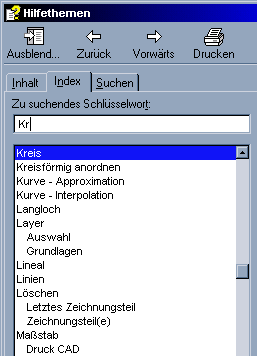
\includegraphics{pic/Suche2.png}

Wenn Sie den richtigen Begriff gefunden haben klicken Sie ihn doppelt an. Im rechten Fenster 
erscheint die Hilfsseite, die das Thema erläutert.

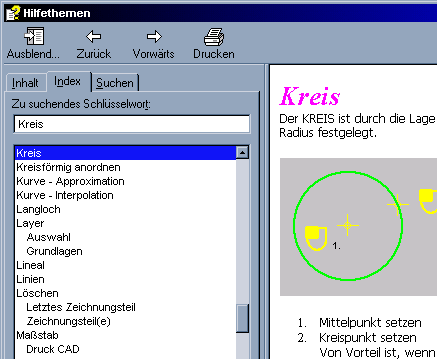
\includegraphics{pic/Suche3.png}

\TRchapter{Grundlagen der Bedienung}{Основные принципы работы}
	\TRsection{Kurzanleitung}{Краткое руководство}
	\TRsection{Bedienprinzip}{Принцип действия}
	\TRsection{Drucken}{Печать}
	\TRsection{Konfiguration von nccad7}{Конфигурирование nccad7}
	\TRsection{Vorlagen}{Шаблоны}
	\TRsection{Das Menü}{Меню}
		\subsection{Ansicht}{Вид}
		\subsection{Datei}{Файл}
		\subsection{Hilfe}{Помощь}
		\subsection{Maschine}{Станок}
		\subsection{Parameter}{Параметры}
		\subsection{Simulation}{Симуляция}
	\TRsection{Die Icons}{Иконки}
		\TRsubsection{Bearbeitung}{Обработка}
			\subsubsection{Drehen}{Стрелять}
			\subsubsection{Eigenschaften ändern}{Изменение свойств}
			\subsubsection{Konstruktionspunkt verschieben}{Перемещение конструкционных
			точек}
			\subsubsection{Kopieren}{Копировать}
			\subsubsection{Korrektur Texte}{Исправление текста}
			\subsubsection{Kreisförmig anordnen}{Круговое выравнивание}
			\subsubsection{Löschen}{Удалить}
			\subsubsection{Löschen Letztes}{Удалить последнюю}
			\subsubsection{Rückgängig Letztes}{Отменить последнее}
			\subsubsection{Skalieren}{Масштабирование}
			\subsubsection{Spiegeln horizontal}{Отразить горизонтально}
			\subsubsection{Spiegeln horizontal mit Kopie}{Отразить горизонтально с
			копией}
			\subsubsection{Spiegeln vertikal}{Зеркалить вертикально}
			\subsubsection{Spiegeln vertikal mit Kopie}{Зеркалить вертикально с копией}
			\subsubsection{Verschieben}{Сдвинуть}
			\subsubsection{Zoom Maßstab}{Зум}
		\subsection{CAD - 3D}
			\TRsubsubsection{Ansicht dreidimensional}{Трехмерное изображение}
			\subsubsection{Plastische Zone Kreis}{Пластичная зона Круг}
			\subsubsection{Plastische Zone Rechteck}{Пластичная зона Прямоугольник}
			\subsubsection{Plastische Zone in STL wandeln}{Пластичная зона Прямоугольник}
			\subsubsection{Schnitt bearbeiten}{Править секцию}
			\subsubsection{Schnitt neu}{Новая секция}
		\TRsubsection{CAD - Besonderes}{CAD - Фичи}
			\subsubsection{Ellipse}{Эллипс}
			\subsubsection{Freihand}{От руки}
			\subsubsection{Kurve Approximation}{Аппроксимация кривых}
			\subsubsection{Kurve Interpolation}{Интерполяция кривых}
			\subsubsection{Mathematische Funktion}{Математические функции}
			\subsubsection{Outline - Generierung}{Outline - генерация}
			\subsubsection{Pad/Bahn - Generierung}{Pad/Bahn - генерация}
			\subsubsection{Schraffieren}{Колодец}
			\subsubsection{Tangente}{Касание}
			\subsubsection{Tangente außen}{Внешнее касание}
			\subsubsection{Tangente innen}{Внутреннее касание}
			\subsubsection{Zahnrad außenverzahnt}{Внешнее зубчатое колесо}
			\subsubsection{Zahnrad innenverzahnt}{Внутреннее зубчатое колесо}
			\subsubsection{Zahnstange}{Зубчатая рейка}
		\TRsubsection{CAD - Standard}{CAD - Стандартный}
			\subsubsection{Bogen} 
			\subsubsection{Gerade}
			\subsubsection{Gravurtext MAX/einzeilig} 
			\subsubsection{Gravurtext MAX/mehrzeilig}
			\subsubsection{Gravurtext TrueType} 
			\subsubsection{Kreis} 
			\subsubsection{Langloch} 
			\subsubsection{Polygon} 
			\subsubsection{Polygon-Generierung} 
			\subsubsection{Punkt} 
			\subsubsection{Rechteck} 
		\DE{\subsection{CAM - Standard}}
		\RU{\subsection{CAM - Стандартные}}
			\subsubsection{Ausspannposition} 
			\subsubsection{Bahnkorrektur} 
			\subsubsection{Insel auflösen}
			\subsubsection{Insel zuweisen} 
			\subsubsection{Kontur auflösen}
			\subsubsection{Kontur generieren}
			\subsubsection{Leitkontur} 
			\subsubsection{Tasche fräsen} 
			\subsubsection{Technologie} 
			\subsubsection{Werkstück - Befestigung} 
			\subsubsection{Werkstück - Nullpunkt} 
		\DE{\subsection{Darstellung}}
		\DE{\subsection{Представление}}
			\DE{\subsubsection{Ansicht Letzte}} 
			\RU{\subsubsection{Последний вид}} 
			\subsubsection{Ausschnitt verschieben} 
			\subsubsection{Ausschnitt wählen} 
			\DE{\subsubsection{Neu darstellen}} 
			\RU{\subsubsection{Новый вид}} 
			\DE{\subsubsection{Tischdarstellung}}
			\DE{\subsubsection{Изображение стола}}
		\DE{\subsection{Dokumentation}}
		\RU{\subsection{Документация}}
			\DE{\subsubsection{Bemaßung horizontal}}
			\RU{\subsubsection{Размер горизонтальный}}
			\DE{\subsubsection{Bemaßung Radius}}
			\RU{\subsubsection{Размер радиус}}
			\DE{\subsubsection{Bemaßung schräg}}
			\RU{\subsubsection{Размер косой}}
			\DE{\subsubsection{Bemaßung vertikal}}
			\RU{\subsubsection{Размер вертикальный}}
			\DE{\subsubsection{Bemaßung Winkel}}
			\RU{\subsubsection{Размер угловой}}
			\DE{\subsubsection{Beschriftung TrueType}} 
			\RU{\subsubsection{Надпись TrueType}} 
			\DE{\subsubsection{Beschriftung MAX/einzeilig}} 
			\RU{\subsubsection{Надпись MAX/однострочный}} 
			\DE{\subsubsection{Beschriftung MAX/mehrzeilig}}
			\RU{\subsubsection{Надпись MAX/многострочный}}
			\DE{\subsubsection{Bearbeiter}}
			\RU{\subsubsection{Редактирование}}
			\DE{\subsubsection{Bearbeiter letzte Änderung}}
			\RU{\subsubsection{Редактирование последней операции}}
			\DE{\subsubsection{Dateiname}}
			\RU{\subsubsection{Имя файла}}
			\DE{\subsubsection{Datum letzte Änderung}}
			\RU{\subsubsection{Datum последней операции}}
			\DE{\subsubsection{Datum aktuell}}
			\RU{\subsubsection{Datum текущей операции}}
			\DE{\subsubsection{Datum Ausdruck}}
% 			\RU{\subsubsection{Datum Ausdruck}}
			\DE{\subsubsection{Datum erstellt}}
			\RU{\subsubsection{Datum создание}}
		\subsection{Einstellungen}
			\DE{\subsubsection{Bezugspunkt}} 
			\RU{\subsubsection{Контрольная точка}} 
			\DE{\subsubsection{Fang}}
			\RU{\subsubsection{Привязка}}
 			\DE{\subsubsection{Layer (Zeichnungslage)}}
 			\RU{\subsubsection{Слой (положение рисунка)}} 
			\DE{\subsubsection{Lineal}}
			\RU{\subsubsection{Линейка}}
			\DE{\subsubsection{Linien}}
			\RU{\subsubsection{Вектор}}
			\DE{\subsubsection{Raster}}
			\RU{\subsubsection{Растр}}
		\DE{\subsection{Information}}
		\RU{\subsection{Информация}}
			\subsubsection{Messen} 
			\subsubsection{Zeichnungsteil-Informationen} 
		\DE{\subsection{Symbole}}
		\RU{\subsection{Символы}}
			\DE{\subsubsection{Symbol auflösen}}
			\RU{\subsubsection{Символ разрешенные}}
			\DE{\subsubsection{Symbol laden}} 
			\RU{\subsubsection{Символ загрузка}} 
			\DE{\subsubsection{Symbol speichern}} 
			\RU{\subsubsection{Символ сохранение}} 
		\DE{\subsection{Umwandlung}}		
		\RU{\subsection{Преобразование}}		
			\subsubsection{Trimmen} 
			\subsubsection{Verlängern} 
			\subsubsection{Trimmen-Verlängern} 
			\subsubsection{Trimmen 2 Teile} 
			\subsubsection{Verlängern 2 Teile} 
			\subsubsection{Auftrennen} 
			\subsubsection{Autom. Trimmen-Verl. (Kontur verfolgen)} 
			\subsubsection{Verdünnen} 
			\subsubsection{Polygon-Generierung} 
			\subsubsection{Konvertieren in Gerade} 
			\subsubsection{Konvertieren in Polygon}
			\subsubsection{Runden} 
			\subsubsection{Runden selektiv} 
			\subsubsection{Fasen} 
			\subsubsection{Fasen selektiv} 
						
\TRchapter{Grundlagen CAD}}
{Основы CAD}}
	\TRsection{CAD - Konstruktionsgrundlagen}}
	{CAD - конструктивные основы}}
	\TRsection{CAD - Kurzanleitung}}
	{CAD - короткое руководство}}
	\TRsection{CAD - 3D Funktionen}}
	{CAD - 3D функции}}
	\TRsection{CAD - Technisches Zeichnen}}
	{CAD - Техническое рисование}}
		\subsection{Dreiseiten-Darstellung}
		\subsection{Räumliche Darstellung}
		\subsection{Arbeiten mit Symbolen}
	\TRsection{Grafik}}
	{Графика}}
		\subsection{Bilder importieren}
		\subsection{Formulare}
	 
\TRchapter{CNC-Fräsmaschinen}{ЧПУ-Фрезерный станок} 
	\section{Inbetriebnahme, Erste Schritte}
	\section{Handsteuerung}
	\section{CNC-Fräsen}
	\section{Teach In - Programmierung} 
	\section{Simulation mit OpenGL} 
	\section{Werkzeug-Korrektur} 
	\section{CAD/CAM-Fräsen} 
		\subsection{Einführungsbeispiel, Prinzip} 
		\subsection{Technologie-Angaben} 
	\section{3D-Fräsen}
		\subsection{Körper aus Rippen und Spanten} 
		\subsection{Plastische Zonen} 
		\subsection{Randzonen} 
		\subsection{STL Grundlagen} 
		\subsection{STL Ebenenbearbeitung} 
		\subsection{STL 4-Achs-Bearbeitung}
	\section{Bearbeitungseinheiten} 
		\subsection{Universal (Metabo)} 
		\subsection{Schnellfrequenz} 
		\subsection{Drehstrom} 	 
	\section{Arbeitshinweise}
		\subsection{WNP verschieben} 
		\subsection{Maschine aufrüsten}
	\section{Hilfsmittel} 
		\subsection{Pratze, Treppenbock} 
		\subsection{Anschlagwinkel} 		 
	\section{Spezialanwendungen} 
		\subsection{Mit Sonderwerkzeugen}
			\subsubsection{Gewindefräser ZBGF} 
		\subsection{Gravuren} 
			\subsubsection{MAX-Schriften} 
			\subsubsection{TrueType-Schriften} 
			\subsubsection{Fortlaufende Zahlen}
			\subsubsection{am Bogen}
		\subsection{Leiterplatten} 
			\subsubsection{Mit nccad entwerfen und fräsen} 
			\subsubsection{Von Layout-Programmen bearbeiten} 
			\subsubsection{Von Layout-Programmen bohren} 
		\subsection{Zahnräder} 
			\subsubsection{Grundlagen} 
			\subsubsection{Bearbeiten} 
			\subsubsection{Praxis} 			
		\subsection{Schneiden} 
			\subsubsection{Schleppmesser} 
		 
\chapter{CNC-Bohrmaschinen} 
\chapter{ЧПУ-Сверлильный станок} 
	\section{Bediengrundlagen}

\chapter{CNC-Drehmaschinen}
	\section{Daten und Fakten} 
	\section{Inbetriebnahme, Erste Schritte} 
	\section{CNC-Drehen} 
	\section{Simulation mit OpenGL} 
	\section{Werkzeugverwaltung} 
	\section{Testhilfen} 
	\section{CAD/CAM-Drehen} 
		\subsection{Prinzip} 
		\subsection{Mehrfachzyklen} 
	\section{Spezialanwendungen} 
		\subsection{Gewinde-Drehen} 
		\subsection{CNC-Zyklen} 
 
\chapter{Dosier-Systeme}
	\section{Grundlagen} 
	\section{Schubdosierung} 
 
\chapter{Automatisierungs-Systeme}
	\section{Grundlagen} 
	\section{Schaltfunktionen während Bewegung} 
 
\chapter{KOSY-Steuerungen} 
	\section{Standard-Ausführung} 
	\section{Wabeco-Ausführung} 

\chapter{Spezial-Funktionen/Programme} 
	\section{Hilfsprogramme} 
		\subsection{Zeichensatz-Editor} 

\chapter{Import/Export} 
	\section{CNC-Programmexport} 
	\section{Postprozessoranpassung} 
	\section{Schnittstellen} 
	\section{2D-Import} 
		\subsection{DXF}
		\subsection{HPGL} 
		\subsection{Nachbearbeitung} 
		\subsection{Scannen und Vektorisieren} 
	\section{3D-Import} 
		\subsection{STL}
	\section{3D-Export} 
		\subsection{STL}

\chapter{Optionen und deren Bedienung} 
	\section{Abtasten}
	\section{Drehen} 
	\section{KOSY Wagen} 
	\section{Mindermengendosierung} 
	\section{Schubdosierung} 
	\section{Spooler} 
	\section{Tiefenregelung} 
	\section{Werkzeuglängenmessung} 
	\section{Werkzeugwechsel} 

\chapter{Umgang mit dem System}
	\section{Service und Wartung} 
		\subsection{Fehlerliste} 
		\subsection{Hotline} 
		\subsection{Massiv-Körper reparieren} 
	\section{Transport} 
		\subsection{Massive Maschinen} 
		\subsection{Paketversand} 
 
\chapter{Anhang}
	\section{Liesmich/Installation} 
	\section{Anschlussbelegung} 
	\section{CAM-Technologien} 
	\section{Dreh-Zyklen} 
	\section{NC-Befehle} 
	\section{NC-Kurzbefehlsliste} 
	\section{Netzwerk-Installation} 
	\section{Tastenbelegung (HotKeys)} 
 
 
\part{ZSE3}

\end{document}